\chapter{Theory and motivation}
\label{chap:prod:theory}

For an observable cross-section \xsec\ of inclusive production of some object 
$P$, $\decay{h_{A}h_{B}}{PX}$, involving two initial-state hadrons $h_{A}$ and 
$h_{B}$, the dominant contribution to a prediction can be expressed as the 
convolution of several terms
\begin{equation}
  \xsec = \sum_{a,b} \sigma_{a,b} \otimes f_{a,A} \otimes f_{b,B},
  \label{eqn:prod:theory:factorisation}
\end{equation}
where the sum runs over all parton types $a$ and $b$ in the respective hadrons 
$h_{A}$ and $h_{B}$; $\sigma_{a,b}$ is the cross-section of the hard partonic 
interaction $\decay{ab}{PX}$; and $f$ is the \ac{QCDPDF} for the interacting 
parton in the respective hadron~\cite{Collins:1989gx,Forte:2013wc}.
The parton-parton cross-sections $\sigma_{a,b}$, for processes such as heavy 
quark pair production via gluon-gluon fusion shown in 
\cref{fig:intro:lhcb:hf_production:gg_fusion}, can be computed using 
perturbative \ac{QCD}.
The computations of the \acp{QCDPDF} involve low-energy processes below the 
\ac{QCD} scale, and so must be evaluated using non-perturbative \ac{QCD} 
instead.
Clearly, the computation of any cross-section at the \ac{LHC} relies on being 
able to evaluate \cref{eqn:prod:theory:factorisation}, including the 
computation of production rates of the Higgs boson and particles beyond the 
\ac{SM}, and hence on a knowledge of the \acp{QCDPDF}.
As the \acp{PDF} cannot be computed from first principles, they must be derived 
be alternate means, and in practice are constrained using measurements of 
cross-sections by experiments.
Additional measurements of cross-sections can constrain the \acp{QCDPDF} 
further, improving their precision.

Parton density functions are parameterised in terms of \bjorkenx, the fraction 
of the total hadron momentum carried by the interacting parton, and 
\pdfqsquared, a measure of momentum transfer and inversely proportional to the 
spatial `scale' at which the hadron can be probed, with a larger \pdfqsquared\ 
corresponding to a finer resolvable structure.
The \ac{QCDPDF} $f(\bjorkenx, \pdfqsquared)$ for a particular hadron is an 
intrinsic property, and so, for example, experimental measurements that can 
constrain the \ac{QCDPDF} in high-energy proton collisions help not only the 
experiments at that collider, but also experiments at other proton colliders.
This is possible as the evolution of the \acp{QCDPDF} over \pdfqsquared\ for a 
given value of \bjorkenx\ is described by the \ac{DGLAP} differential 
equations~\cite{Gribov:1972ri,Dokshitzer:1977sg,Altarelli:1977zs}.
Measuring a wide range of \bjorkenx\ is important as the individual 
contributions to the total \ac{QCDPDF}, such as from the gluons and the valence 
quarks, vary strongly as a function of \bjorkenx, as shown in 
\cref{fig:prod:theory:pdf_sets}.
The usage of the \ac{DGLAP} equations requires an initial \ac{QCDPDF} from 
which to evolve to different scales, however, as the dependence on \bjorkenx\ 
cannot be computed perturbatively.
Such inputs were first provided by \ac{DIS} experiments, which probe the proton 
structure by colliding leptons and protons.
The subsequent evolution of the \acp{PDF} have been driven by additional 
experimental measurements, and by an improved theoretical understanding of the 
use of the perturbative expansion that must be employed when solving the 
\ac{DGLAP} equations.

The treatment of experimental inputs is a matter of debate, as there are 
somewhat arbitrary choices to be made on what experimental inputs should be 
used, and on how the various experimental uncertainties should be treated.
As a result, different groups of theorists provide so-called `\ac{QCDPDF} 
sets', which differ not only in the treatment of the inputs, but also in the 
treatment of the \emph{theoretical} uncertainties.
These include, for example, the choice of order to which the perturbation 
series are evaluated, and whether the value of the perturbation series scale is 
a parameter of the fit or if it is fixed.
For heavy flavour production, additional uncertainties arise from the choice of 
\emph{fragmentation function} models~\cite{Kneesch:2007ey}, which describe how 
the heavy quarks transition into the observed hadrons, a factor which is not 
included in the factorisation theorem shown in 
\cref{eqn:prod:theory:factorisation}.\footnotemark\
The different \ac{QCDPDF} sets can be used to compute different cross-section 
predictions, and so further experimental measurements can help to distinguish 
between predictions.

\footnotetext{%
  The fragmentation functions are generally assumed to be process independent, 
  e.g.\ they are the same for heavy flavour hadron production from \qqbar\ 
  production at both $\Pelectron\APelectron$ and $\Pproton\Pproton$ colliders.
  They cannot be computed perturbatively, and are extracted from experimental 
  measurements.
}

\begin{figure}
  \begin{subfigure}[b]{0.5\textwidth}
    \centering
    \begin{tikzpicture}
  \node[anchor=south west, inner sep=0] (image) at (0, 0) {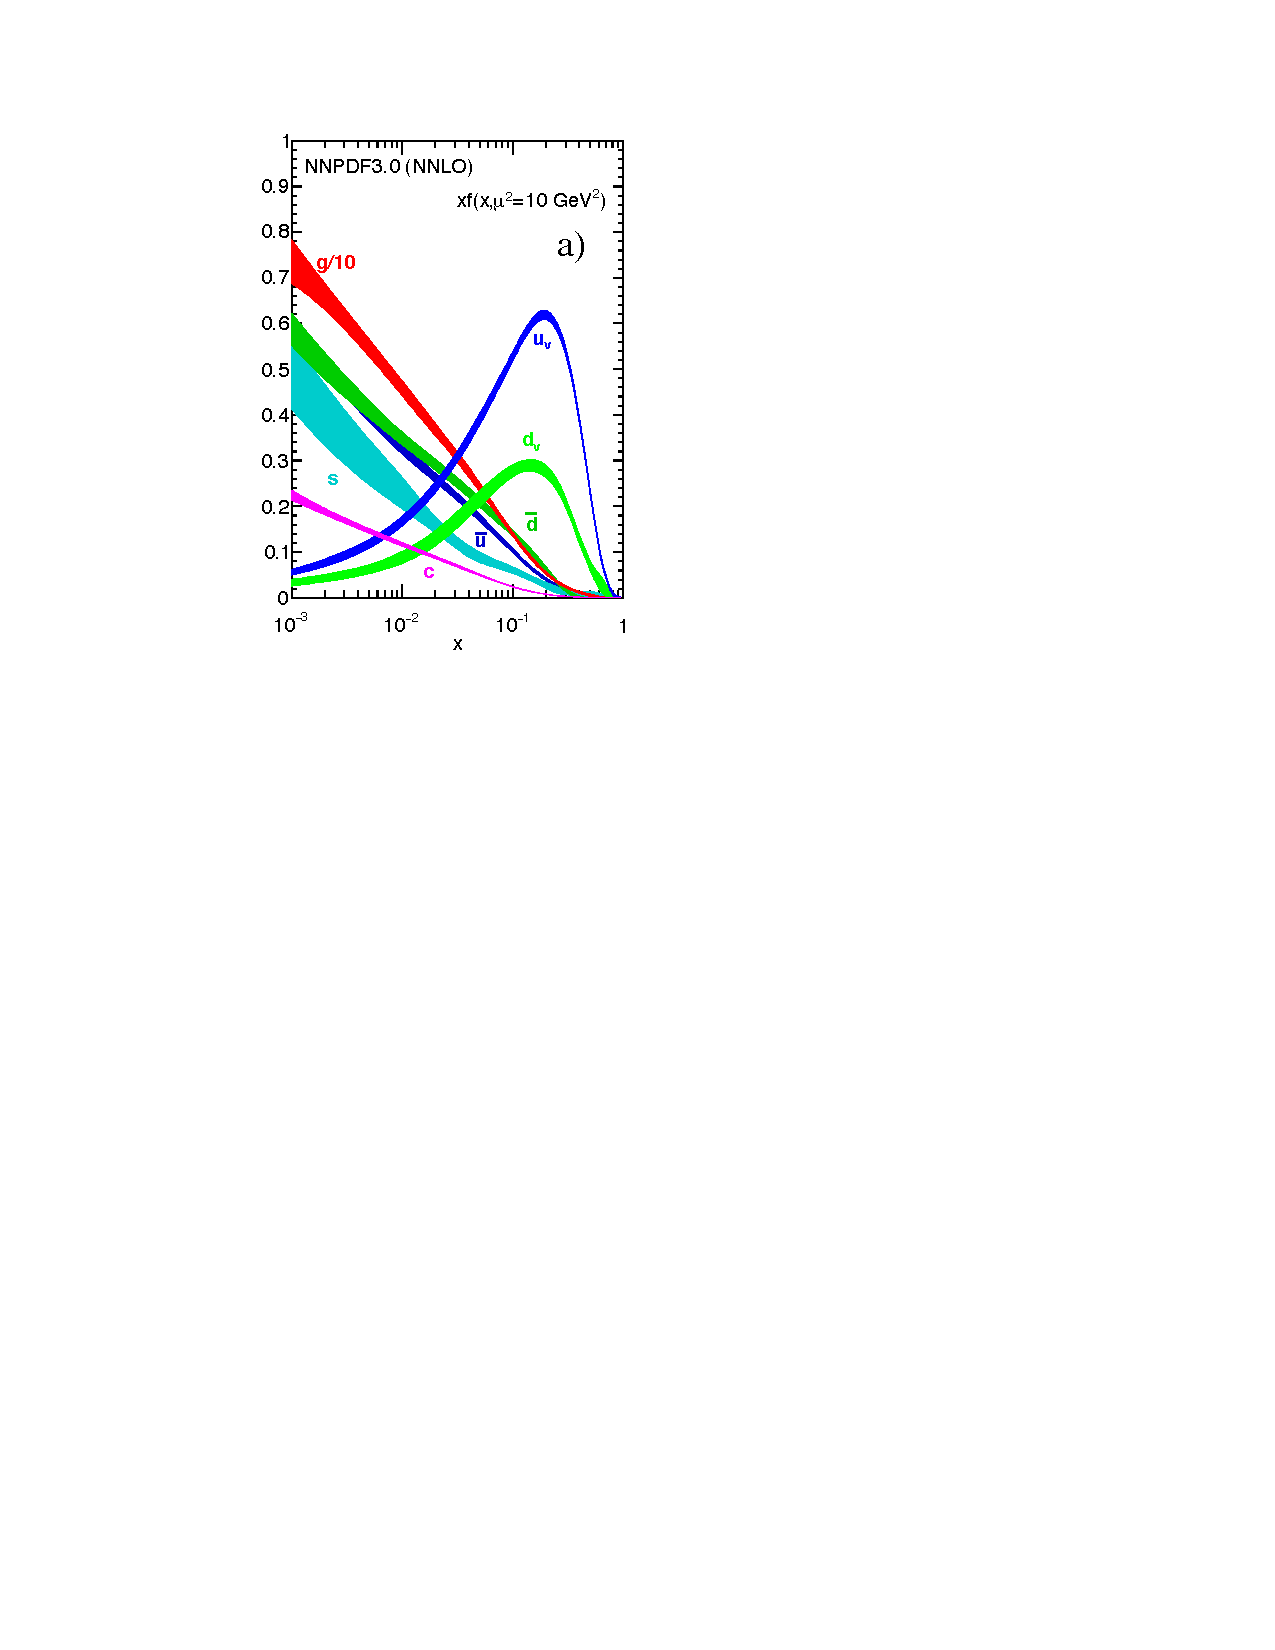
\includegraphics[width=\textwidth]{production/pdf_sets_low_qsquared}};
  \begin{scope}[x={(image.south east)}, y={(image.north west)}]
    % Grid to help find coordinates on the image
    % \draw[step=0.02, gray, very thin] (0, 0) grid (1, 1);
    % Box to cover 'a)' label
    \path[fill=white] (0.8, 0.74) rectangle (0.9, 0.82);
  \end{scope}
\end{tikzpicture}

    \caption{Low \pdfqsquared}
    \label{fig:prod:theory:pdf_sets:low_qsquared}
  \end{subfigure}
  \begin{subfigure}[b]{0.5\textwidth}
    \centering
    \begin{tikzpicture}
  \node[anchor=south west, inner sep=0] (image) at (0, 0) {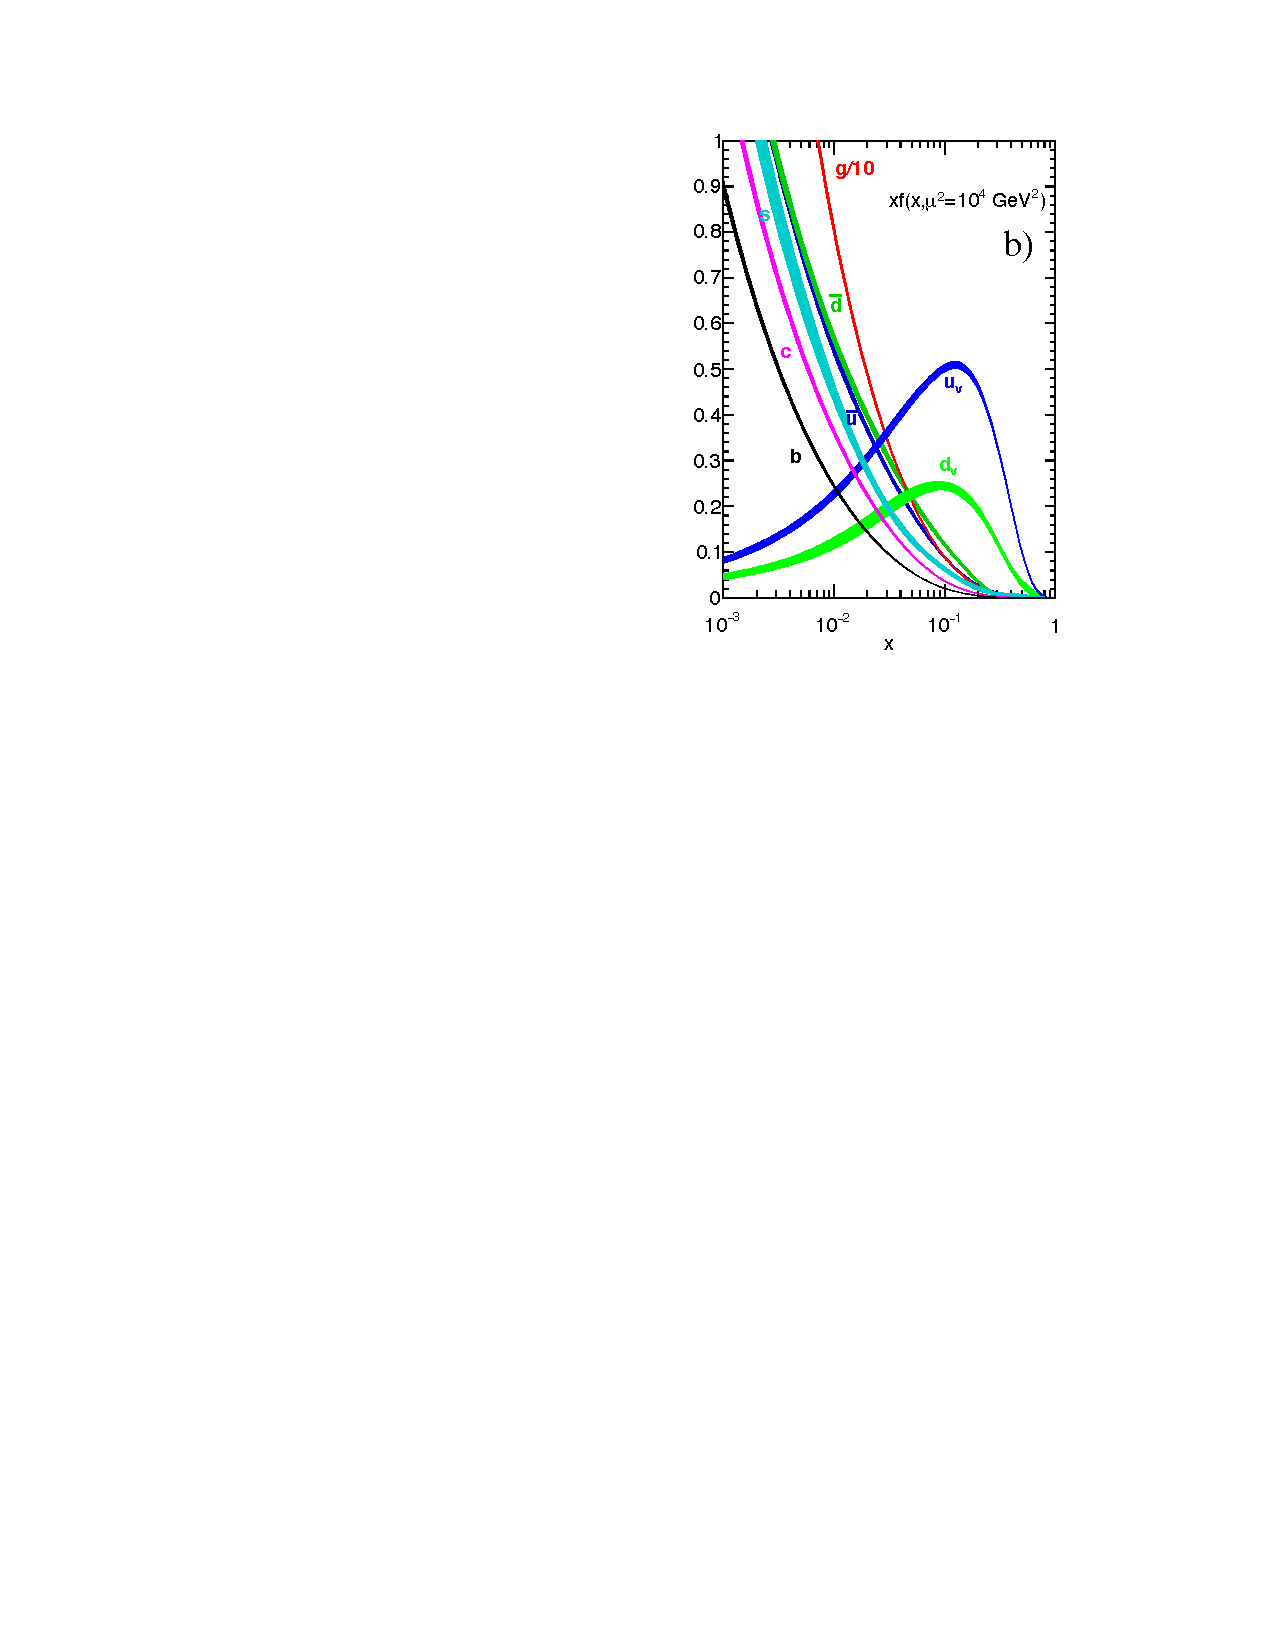
\includegraphics[width=\textwidth]{figures/production/pdf_sets_high_qsquared}};
  \begin{scope}[x={(image.south east)}, y={(image.north west)}]
    % Grid to help find coordinates on the image
    % \draw[step=0.02, gray, very thin] (0, 0) grid (1, 1);
    % Box to cover 'b)' label
    \path[fill=white] (0.82, 0.74) rectangle (0.94, 0.82);
  \end{scope}
\end{tikzpicture}

    \caption{High \pdfqsquared}
    \label{fig:prod:theory:pdf_sets:high_qsquared}
  \end{subfigure}
  \caption{%
    Sets of proton \aclp{QCDPDF} for low \pdfqsquared\ 
    (\subref*{fig:prod:theory:pdf_sets:low_qsquared}) and high \pdfqsquared\ 
    (\subref*{fig:prod:theory:pdf_sets:high_qsquared}), illustrating both 
    \bjorkenx\ and \pdfqsquared\ dependence~\cite{PDG2014}.
    Each band represents the \ac{QCDPDF} for a specific parton, as a function 
    of \bjorkenx, shown on the $x$-axis.
    The $\Pup_{\text{v}}$ and $\Pdown_{\text{v}}$ bands show the contributions 
    from the valance quarks, the \Pgluon band shows the gluon contribution, and 
    the other bands show the contribution from flavour-specific sea quarks.
  }
  \label{fig:prod:theory:pdf_sets}
\end{figure}

\subsection{Experimental input}
\label{chap:prod:theory:pdfs:inputs}

Today, inputs from both \ac{DIS} and hadron-hadron collider experiments serve 
to constrain proton \acp{QCDPDF} over a wide range of \bjorkenx\ and 
\pdfqsquared\ values.
The most recent and most powerful \ac{DIS} measurements have been made by the 
\hone\ and \zeus\ collaborations at the \hera\ $\Pe\Pproton$ 
collider~\cite{Abramowicz:1900rp}.
However, these measurements are largely constrained to measure values of 
\bjorkenx\ above \num{e-4}, leading to large uncertainties at low \bjorkenx.
This low-\bjorkenx\ region is particularly interesting to study not only 
because the current \ac{QCDPDF} uncertainties there are large, but also because 
it is where both the gluon and the sea quark contributions to the total 
\ac{QCDPDF} are large, as shown in \cref{fig:prod:theory:pdf_sets}, and so 
low-\bjorkenx\ measurements probe phenomenologically different processes.

In a hard \decay{2}{2} process, such as $\Pgluon\Pgluon$ fusion or \qqbar\ 
annihilation to a heavy quark pair, the extent in \bjorkenx\ that can be probe 
with heavy flavour hadron production measurements is given by
\begin{equation}
  {\bjorkenx}_{\text{min}} = e^{\pm\rapidity}\frac{%
    \sqrt{\pT^{2} + m_{\Pquark}^{2}}
  }{%
    \sqrts
  },
  \label{fig:prod:theory:hf_bjorkenx}
\end{equation}
where \rapidity\ and \pT\ parameterise the hadron kinematics, and $m_{q}$ is 
the mass of the heavy quark in the hadron under study~\cite{Zenaiev:2015rfa}.
There is then a wide range of \bjorkenx\ values that can be probed at proton 
colliders, with the highest sensitivity to low \bjorkenx\ provided by charm 
production measurements.\footnotemark\
At the \ac{LHC}, the dominant production mechanism is gluon-gluon fusion, as 
depicted in \cref{fig:intro:lhcb:hf_production:gg_fusion}, and so measurements 
at the \ac{LHC} are able to provide particularly strong constraints on the 
gluon densities.
Charm cross-sections have been measured in the $|\rapidity| < 0.5$ region for 
$\pT > \SI{1}{\GeVc}$ at \sqrtseq{2.76}\ and \sqrtseq{7}\ by the \alice\ 
collaboration~\cite{Abelev:2012sx,ALICE:2012ik,ALICE:2011aa},
and for pseudorapidity $|\Eta| < 2.1$ in the \pT\ region $3.5 < \pT < 
\SI{100}{\GeVc}$ at \sqrtseq{7} by the \atlas\ 
collaboration~\cite{Aad:2015zix}.

\footnotetext{%
  The charm quark mass is four times less than that of the bottom quark.
}

Measurements of charm production at \sqrtseq{7}\ were made by the \lhcb\ 
collaboration~\cite{LHCb-PAPER-2012-041}.
By \cref{fig:prod:theory:hf_bjorkenx}, measurements of charm hadron production 
for \pT\ values of the order of \SI{1}{\GeVc} at the lowest rapidities 
accessible to \lhcb\ can probe \bjorkenx\ values down to the order of \SI{e-6}, 
with lower values possible for measurements at a higher \sqrts, as shown in 
\cref{fig:prod:theory:prosa_x_regions}.
These measurements, along with similar measurements of beauty hadron production 
at \lhcb~\cite{LHCb-PAPER-2013-004} and the aforementioned \hone\ and \zeus\ 
measurements, have been used by the \prosa\ 
collaboration~\cite{Zenaiev:2015rfa} to constrain the proton \aclp{QCDPDF}, 
where they see a significant reduction on the gluon \ac{QCDPDF} uncertainty 
when including the \lhcb\ data, with respect to using the \hera\ data only, as 
shown in \cref{fig:prod:theory:prosa_gluon_pdf_fit}.
It is expected that additional measurements, at \sqrtseq{13}, can be used to 
further reduce the gluon \ac{QCDPDF} uncertainties~\cite{Gauld:2015yia}.

% \begin{figure}
%   \centering
%   \begin{tikzpicture}
  \begin{feynman}[scale=1.25,transform shape]
    \vertex (a);
    \vertex [right=of a] (b);

    \vertex [above left=of a] (i1) {\(\Pgluon\)};
    \vertex [below left=of a] (i2) {\(\Pgluon\)};

    \vertex [above right=of b] (f1) {\(\Pquark\)};
    \vertex [below right=of b] (f2) {\(\APquark\)};
    % Vertex in between b and f2, for the radiative gluon
    \vertex (bf1) at ($(b)!0.5!(f2)$);
    \vertex [right=of b] (f3);

    \diagram* [large] {
      (a) -- [gluon, edge label=\(\Pgluon\)] (b),
      (i1) -- [gluon] (a),
      (i2) -- [gluon] (a),
      (b) -- [fermion] (f1),
      (f2) -- [fermion] (b),
      (bf1) -- [gluon, edge label=\(\Pgluon\)] (f3),
    };
  \end{feynman}
\end{tikzpicture}

%   \caption{%
%     Feynman diagram of \qqbar\ pair production via \qqbar\ annihilation.
%   }
%   \label{fig:prod:theory:qqbar_annihilation}
% \end{figure}

\begin{figure}
  \centering
  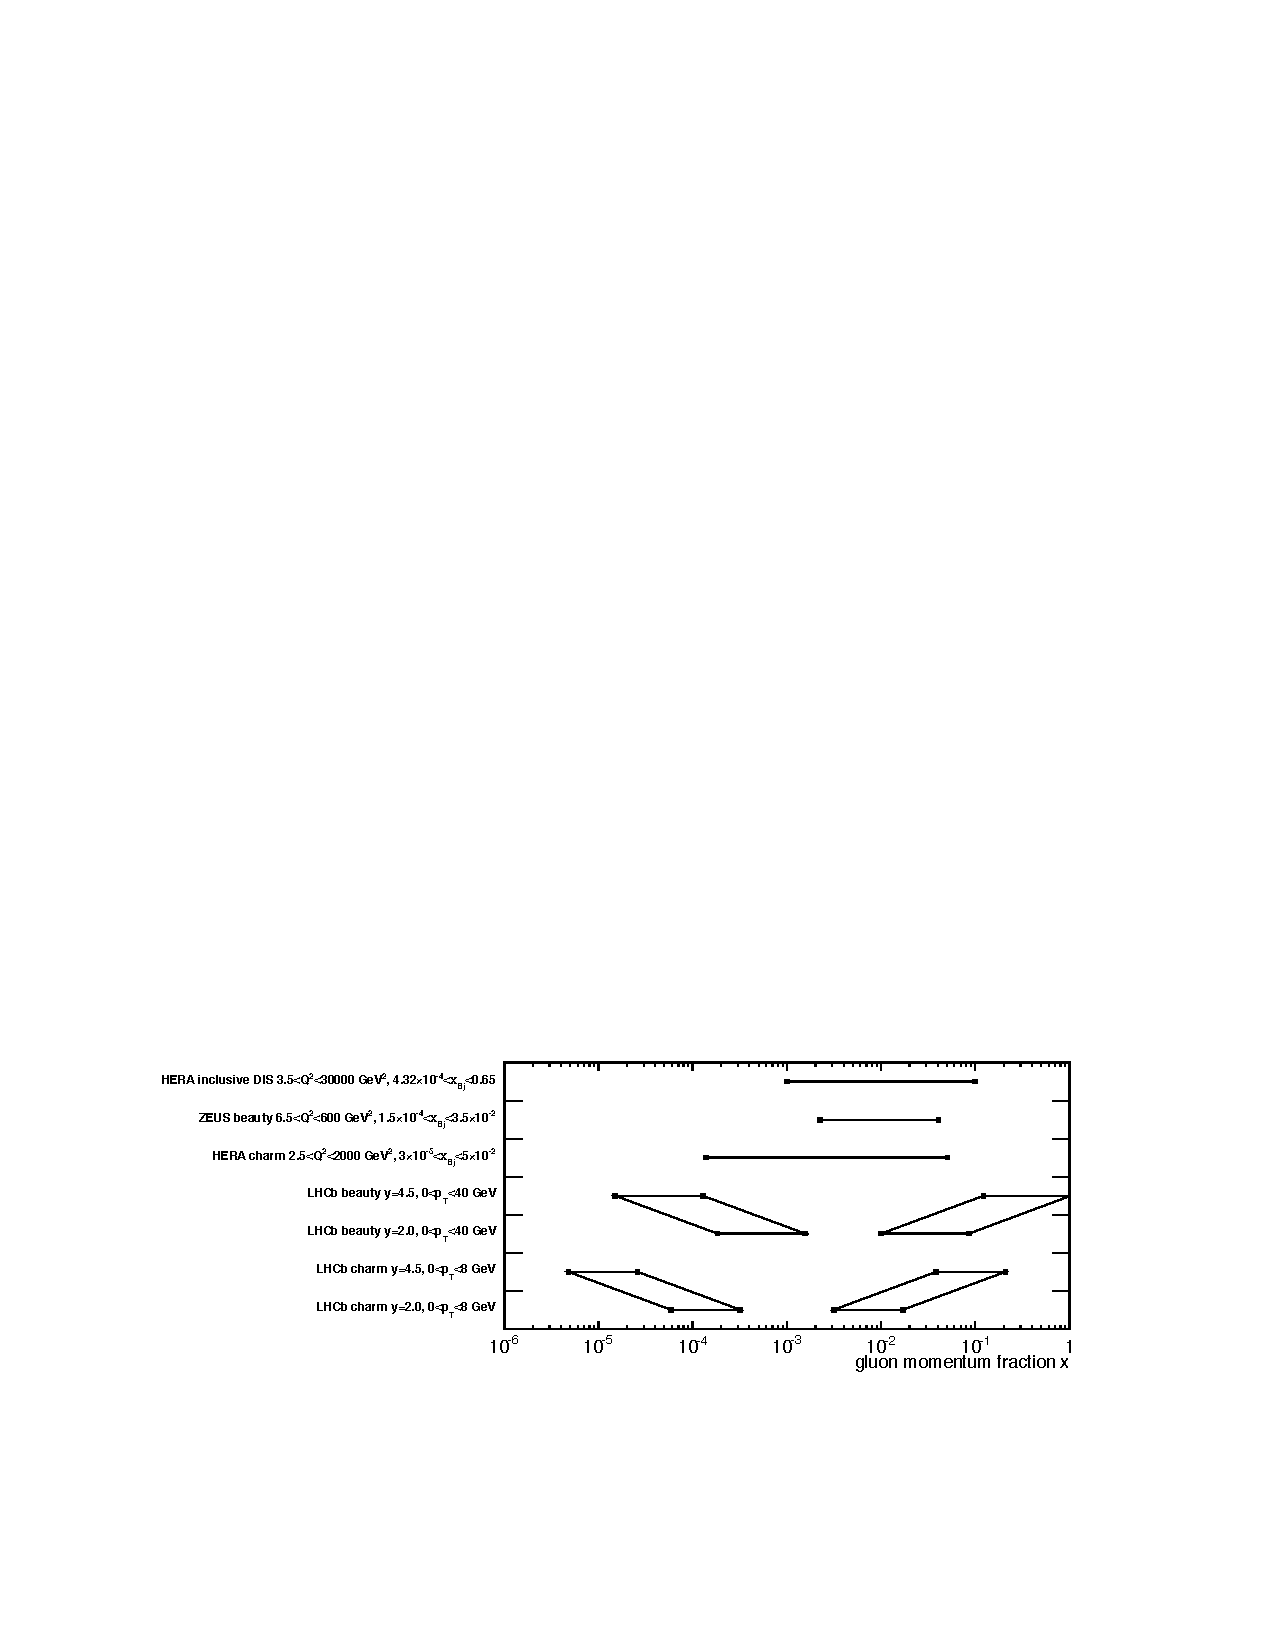
\includegraphics[width=\textwidth]{production/prosa_x_regions}
  \caption{%
    Regions of proton momentum fraction \bjorkenx, on the $x$-axis, probed by 
    different experiments, indicated on the $y$-axis~\cite{Zenaiev:2015rfa}.
  }
  \label{fig:prod:theory:prosa_x_regions}
\end{figure}

\begin{figure}
  \centering
  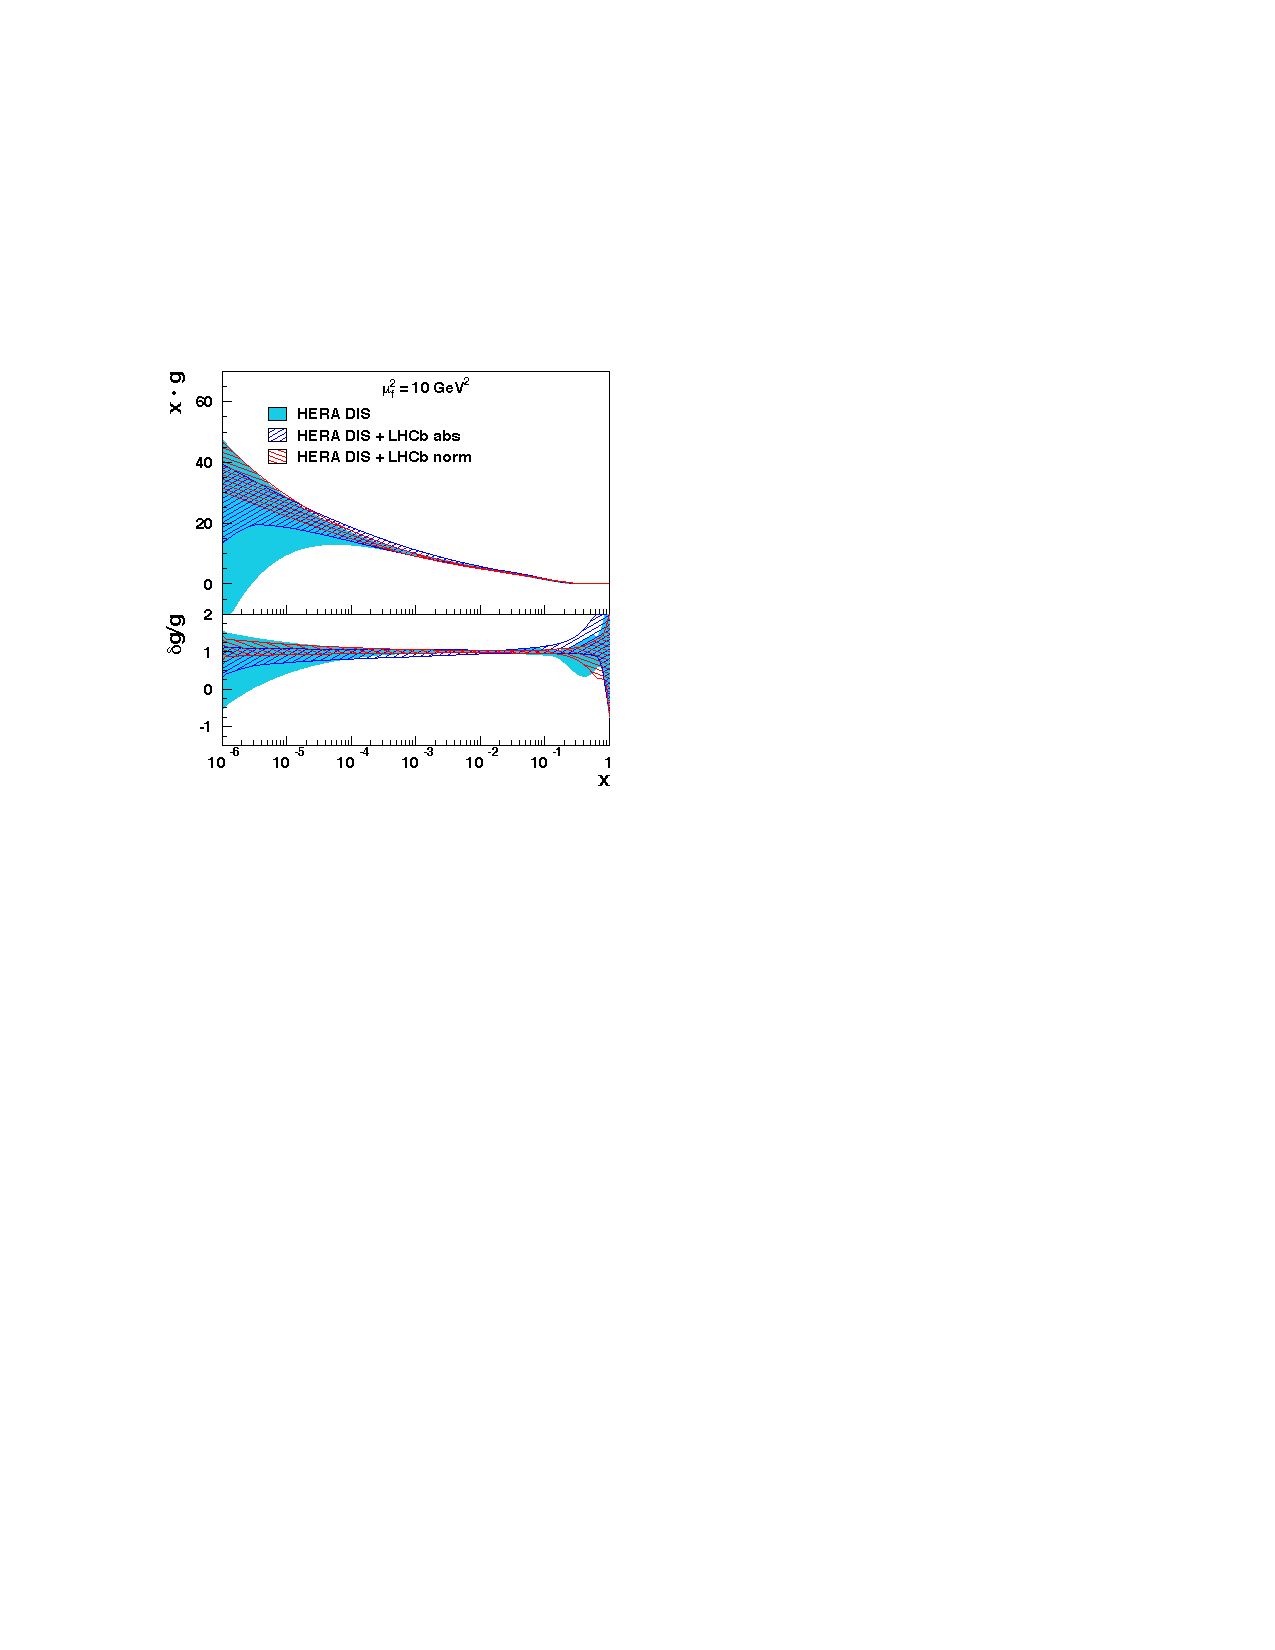
\includegraphics[width=\textwidth]{production/prosa_gluon_pdf_fit}
  \caption{%
    Gluon \acp{QCDPDF} after fitting to experimental 
    data~\cite{Zenaiev:2015rfa}.
    The $x$-axis shows the proton momentum fraction \bjorkenx, the $y$-axis on 
    the top plot shows the gluon \ac{QCDPDF} density, and the $y$-axis on the 
    bottom bottom shows the relative uncertainty on the model.
    The solid band shows the fit when only using the \hera\ measurements as 
    inputs, whilst the hatced bands show the fit when using both the \hera\ and 
    \sqrtseq{7}\ \lhcb\ measurements.
  }
  \label{fig:prod:theory:prosa_gluon_pdf_fit}
\end{figure}

\section{Atmospheric neutrino fluxes}
\label{chap:prod:theory:neutrinos}

The constraints imposed on the proton \acp{QCDPDF} are also useful in 
atmospheric neutrino experiments.
The \icecube\ collaboration aims to measure highly energetic neutrinos of 
astrophysical origin with energies up to the \si{\peta\eV} scale, using the 
IceCube Neutrino Observatory~\cite{Achterberg:2006md}.
This is done to shed light on the mystery of ultra-high-energy cosmic rays 
(protons) whose source is unknown but should also produce similarly energetic
neutrinos.
The so-called conventional neutrino flux constitutes one of the backgrounds for 
astrophysical neutrino experiments.
This is made by cosmic rays interacting in the atmosphere and producing pions 
and kaons, which then decay to final states containing neutrinos.
However, for the high energies the \icecube\ detector is sensitive to, 
beginning at around \SI{100}{\GeV}, this background is suppressed.
The long lifetime of the mesons increases the probability they will interact 
with the atmosphere in flight, losing energy through hadronic interactions, 
hence reducing the energy spectrum of the resulting neutrinos.
However, an additional background comes from the production of charm hadrons in 
the atmosphere, which, with their comparatively short lifetimes, lose very 
little energy in flight, and so the neutrino spectrum from charm decays is very 
similar to the cosmic ray energy spectrum.
The neutrinos produced in the charm decays can interact with the detector in a 
similar manner to the signal and exhibit a similar energy spectrum.
It is then of key importance that the amount of expected background from these 
decays is known, else neutrinos from charm decays may be misinterpreted as 
neutrinos from astrophysical sources.
This contamination can be estimated by predicting the proton-proton 
cross-sections (between the cosmic ray and the nuclei in the atmosphere).

Colliding equal-energy proton-proton beams at a centre-of-mass energy of 
\SI{13}{\TeV} is equivalent to directing a proton beam of energy 
\SI{100}{\peta\eV} into a fixed target, as $\sqrts \approx 
\sqrt{2E_{\Pproton}m_{\Pproton}}$, where $E_{\Pproton}$ is the energy of the 
proton beam and $m_{\Pproton}$ is the proton mass.
Hence, measuring charm cross-sections at \sqrtseq{13}\ at the \ac{LHC} can 
provide constraints on the expected rate of charm production in the atmosphere 
produced by extremely high-energy cosmic rays.
Indeed, the measurements made by \lhcb\ at \sqrtseq{7}\ have already been used 
to that effect, and additional measurements at \SI{13}{\TeV} can help 
further~\cite{Gauld:2015yia,Bhattacharya:2015jpa}.

\section{Cross-section comparisons with theory}
\label{chap:prod:theory:comparisons}

A useful check of \acp{QCDPDF} constrained with past experimental data is to 
compute cross-section predictions using them, for comparison with new 
experimental results.
This was done in the previous \lhcb\ open charm cross-section analysis, shown 
in \cref{fig:prod:theory:comparisons:7tev}, where at low \pT\ the data 
generally lie above the theory prediction.
Additional measurements can help in the understanding of these discrepancies.

For the analysis presented in this \namecref{chap:prod}, a measurement of charm 
production at \sqrtseq{13}, three theory groups have provided predictions for 
the double differential cross-sections.
Each set of predictions is computed at next-to-leading order in the strong 
coupling constant \alphas\ (that is, up to the first power of $\alphas$), and 
includes uncertainties from: the factorisation scale dependence, which is the 
scale \pdfqsquared\ at which the perturbative expansion was made; and the 
renormalisation scale, which is the scale at which the expansion is 
renormalised to remove ultraviolet divergences.
These affect both the evaluation of the partonic cross-sections and the 
evolution of the \ac{QCDPDF} sets with the \ac{DGLAP} equations.

The \nnpdfl\ predictions~\cite{Gauld:2015yia} use a \ac{QCDPDF} set that 
includes the constraints from the \sqrtseq{7}\ \lhcb\ 
measurement~\cite{LHCb-PAPER-2012-041}, and are provided for all \pTy\ bins for 
\PDz and \PDp mesons.
The \ac{GMVFNS} predictions~\cite{Kniehl:2012ti} are provided for $\pT > 
\SI{3}{\GeVc}$ for all mesons under study, and use the CT10 \ac{QCDPDF} set.
These predictions include a factor to account for the \cToHc\ transition 
probability, obtained by convolving the \decay{\ccbar}{\PHc} cross-sections 
with the appropriate fragmentation functions.
Finally, \ac{FONLL} predicitions~\cite{Cacciari:2015fta} using the \nnpdf\ 
\ac{QCDPDF} sets are provided for for the full \pTy\ phase space for \PDz, 
\PDp, and \PDstarp mesons.
The \fonll\ predictions assume a unit \cToHc\ transition probability, and so 
are multiplied by the fragmentation fractions in 
\cref{tab:prod:introduction:fragmentation_fractions} for comparison with the 
measurements.
The comparison of these predictions with the data will be given in 
\cref{chap:prod:results}.

\begin{figure}
  \centering
  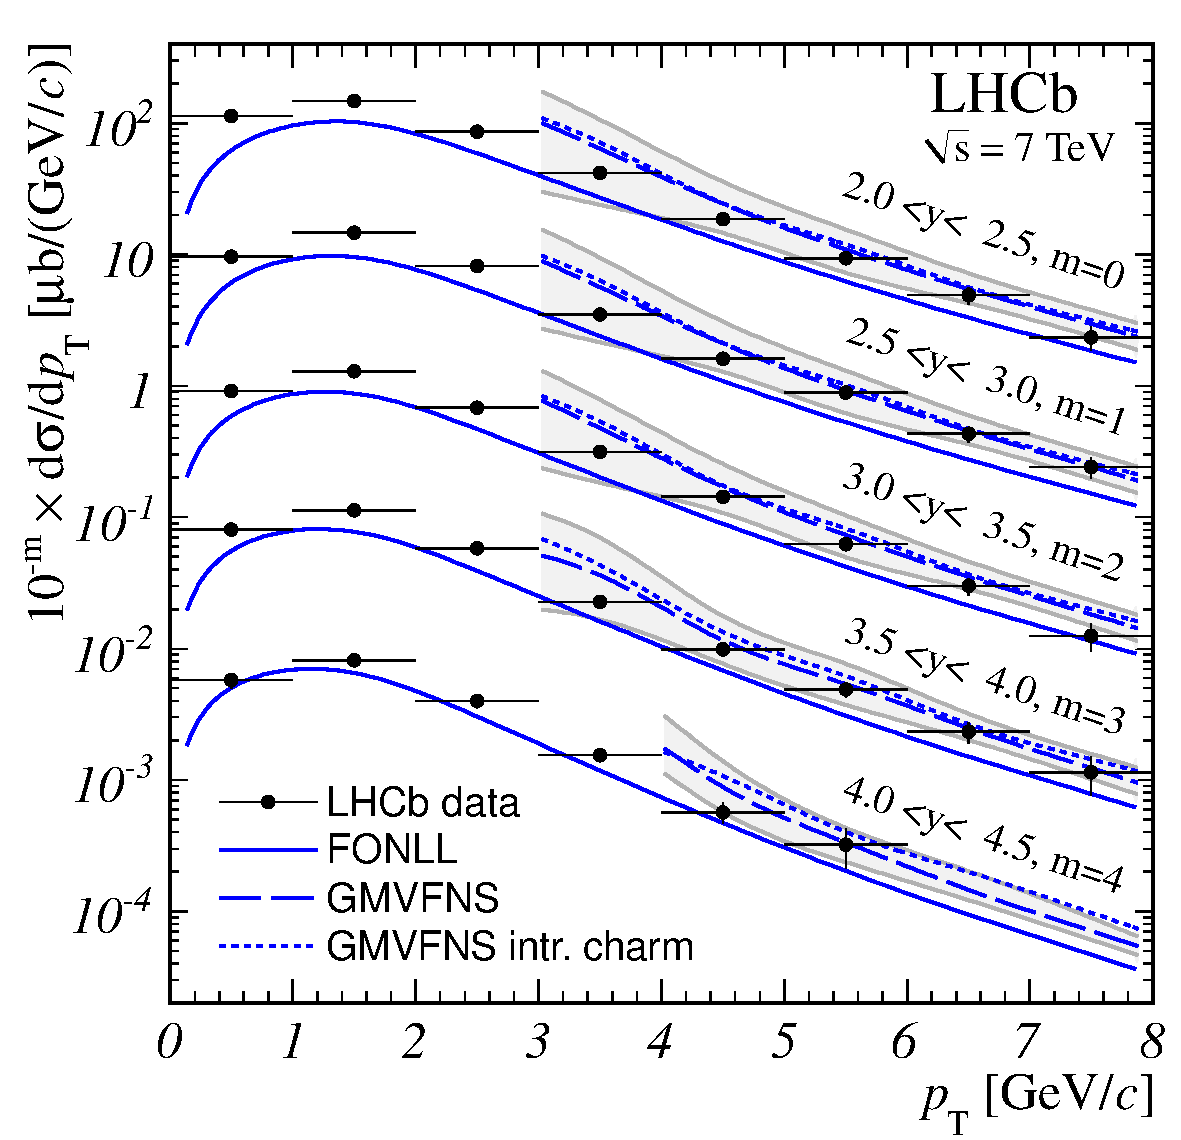
\includegraphics[width=\textwidth]{production/lhcb_dz_xsec_7tev}
  \caption{%
    Prompt \PDzero production rates, measured using the \lhcb\ detector with 
    proton-proton data taken at \sqrtseq{7}~\cite{LHCb-PAPER-2012-041}, in 
    \pTy\ bins.
    The $x$-axis shows the \pT\ of the \PDzero, and the measurements are offset 
    by a multiplicative factor based on the rapidity bin.
  }
  \label{fig:prod:theory:comparisons:7tev}
\end{figure}
